\section{Introduction}
$K$-mer counting is a seemingly relatively straightforward process. Given a sequence $X = \{x_1,\dots,x_L\}$ of length $L$, for each position $i\in 1\leq i\leq \left(L-k+1\right)$ within the sequence, a sub-string is sliced from $[i,i+k)$. Where ``[" indicates inclusion, and ``)" indicates non-inclusive. A hash-map, or dictionary as known within Python, then saves the count for each $k$-mer as encountered in $X$. In many applications, the frequency of each $k$-mer would be calculated by dividing each $k$-mer count by the total number of $k$-mers, \emph{i.e.} $L-k+1$. 

SEEKR differs from this approach in that the algorithm adjusts from the non-uniformity of $k$-mers within our genome. Some $k$-mers are more, or less, frequent than others solely due to mononucleotide frequencies within the genome. Therefore, the enrichment for already common $k$-mers, or depletion of rare $k$-mers, are not informative unless it is known if they are significantly more enriched than background. To account for this, SEEKR calculates a $z$-score for each $k$-mer rather than a frequency.

The $z$-score is calculated by first calculating the $k$-mer frequencies within some reference set of sequences, \emph{e.g.} the transcriptome. From this reference set of $k$-mer frequencies, the mean frequency of each $k$-mer $\mu_j$ and the standard deviation of each $k$-mer $\sigma_j$ is calculated. 

For each $k$-mer frequency $j$ within a sequence $X$, $X_j$ has a $z$-score $X^*_j$: 

\begin{equation}
    X_j^* = \frac{X_j-\mu_j}{\sigma_j}
    \label{eq:zscore}
\end{equation}


We observed when studying the $k$-mer similarities between XIST and RSX that these $z$-scores were approximately log-normally distributed. For the analysis within that paper, we transformed $z$-scores as outlined in 2.X.X. However, we sought to perform a more rigorous analysis of different methodologies for adjusting $k$-mer counts. This chapter outlines the methods that we used and their results. 

\section{Results} 

\subsection{$k$-mer counts are log-normally distributed}
\begin{figure}[h!]
\centering
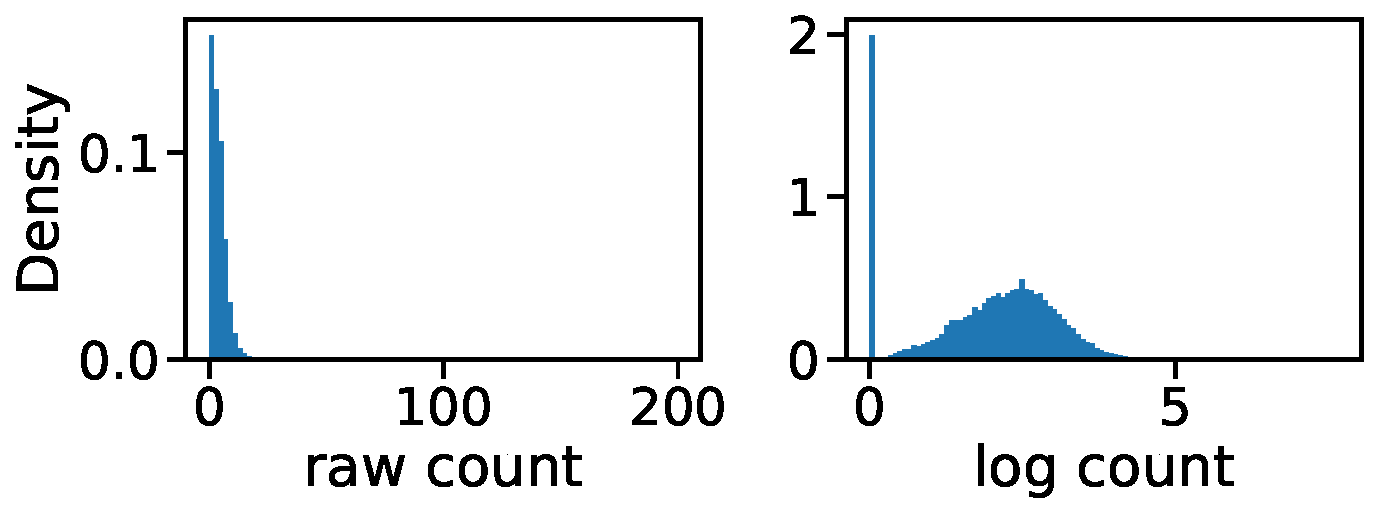
\includegraphics[width=\textwidth]{images/kmers_log_dist.pdf}
\caption{$k$-mer counts are log-normally distributed. A) The frequency of $k$-mer counts over all $k$-mers, over all annotated transcripts in the human genome. B) The distribution in (A), with log-transformed counts.}
\label{fig:logdist}
\end{figure}

\subsection{$k$-mer counting methodologies}

\subsubsection{Row-wise addition of 1 to z-scores}

\begin{table}[h!]
\begin{tabular}{llllll}
&MXA & MXB                   & MXC                  & HXD                  & MXE                                  \\
KR1 & -0.017 & 0.327   & 0.042  & 0.197    & -0.163 \\
KR2 & 0.088   & -0.124 & -0.120 & -0.009 & 0.147 \\
KR3 & -0.079  & -0.090 & 0.016 & -0.022 & 0.246 \\
KR4 & 0.214    & -0.110 & -0.066  & 0.115   & 0.404
\end{tabular}
\end{table}

\subsubsection{Column-wise addition of 1 to z-scores}
\begin{table}[h!]
\begin{tabular}{llllll}
&MXA & MXB                  & MXC                   & HXD                 & MXE                                      \\
KR1 & -0.048 & 0.348    & 0.093 & 0.284  & -0.098 \\
KR2 & 0.057  & -0.046 & 0.034 & 0.201 & 0.261  \\
KR3 & -0.061 & -0.015 & 0.144 & 0.173 & 0.347  \\
KR4 & 0.147   & -0.094  & 0.044 & 0.241 & 0.451 
\end{tabular}
\end{table}

\subsubsection{Sprague et al. 2019}

\begin{table}[h!]
\begin{tabular}{llllll}
&MXA & MBX                  & MXC                  & HXD                  & MXE                                        \\
KR1 & -0.021 & 0.325   & 0.038 & 0.193   & -0.163 \\
KR2 & 0.084  & -0.122  & -0.122 & -0.013 & 0.145  \\
KR3 & -0.077   & -0.093 & 0.014 & -0.023 & 0.249   \\
KR4 & 0.210   & -0.114 & -0.068 & 0.112   & 0.398
\end{tabular}
\end{table}

\subsubsection{Kirk et al. 2018}

\begin{table}[h!]
\begin{tabular}{llllll}
&MXA & MXB                   & MXC                  & HXD                   & MXE                                         \\
KR1 & -0.048 & 0.266   & 0.001 & 0.146    & -0.117 \\
KR2 & 0.085   & -0.089  & -0.111  & -0.024 & 0.147  \\
KR3 & -0.041 & -0.119   & -0.009 & -0.021 & 0.267   \\
KR4 & 0.180   & -0.114 & -0.081  & 0.087   & 0.294 
\end{tabular}
\end{table}

\subsubsection{+1 Raw Count, Length Normalize, log transform}

\begin{table}[h!]
\begin{tabular}{llllll}
&MXA & MXB                  & MXC                  & HXD                  & MXE                                         \\
KR1 & -0.068 & 0.232    & 0.024  & 0.181   & -0.179 \\
KR2 & -0.074 & -0.295 & -0.087 & 0.071  & 0.126  \\
KR3 & -0.170 & -0.170 & 0.063   & 0.001 & 0.205  \\
KR4 & 0.119  & -0.175  & -0.014 & 0.148   & 0.387
\end{tabular}
\end{table}

\subsubsection{+1 Raw count, length normalize, x1000, log transform}

\begin{table}[h!]
\begin{tabular}{llllll}
&MXA & MXB                  & MXC                 & HXD                   & MXE                                         \\
KR1 & -0.068 & 0.232 & 0.024   & 0.181   & -0.179 \\
KR2 & -0.074 & -0.295 & -0.087  & 0.071    & 0.126  \\
KR3 & -0.170  & -0.170 & 0.063    & 0.001 & 0.205  \\
KR4 & 0.119  & -0.175 & -0.014 & 0.148   & 0.387 
\end{tabular}
\end{table}

\subsubsection{Length normalize, +1, log transform}

\begin{table}[h!]
\begin{tabular}{llllll}
&MXA & MXB                   & MXC                  & HXD                   & MXE                                         \\
KR1 & -0.048  & 0.268    & 0.001 & 0.147    & -0.118 \\
KR2 & 0.084   & -0.089 & -0.111  & -0.025  & 0.147  \\
KR3 & -0.042 & -0.120 & -0.008 & -0.022 & 0.266   \\
KR4 & 0.175   & -0.116 & -0.081  & 0.088    & 0.296
\end{tabular}
\end{table}

\subsubsection{adding 1 to all counts after to length normalization then multiplying by 1000 and then log transforming,}

\begin{table}[h!]
\begin{tabular}{llllll}
&MXA & MXB                   & MXC                  & HXD                  & MXE                                        \\
KR1 & -0.013 & 0.335  & 0.059  & 0.200  & -0.163 \\
KR2 & 0.039   & -0.152 & -0.080  & -0.007 & 0.135  \\
KR3 & -0.102   & -0.067 & 0.076  & -0.025 & 0.220   \\
KR4 & 0.249   & -0.078 & 0.015 & 0.150  & 0.431 
\end{tabular}
\end{table}

\begin{figure}[h]
\centering
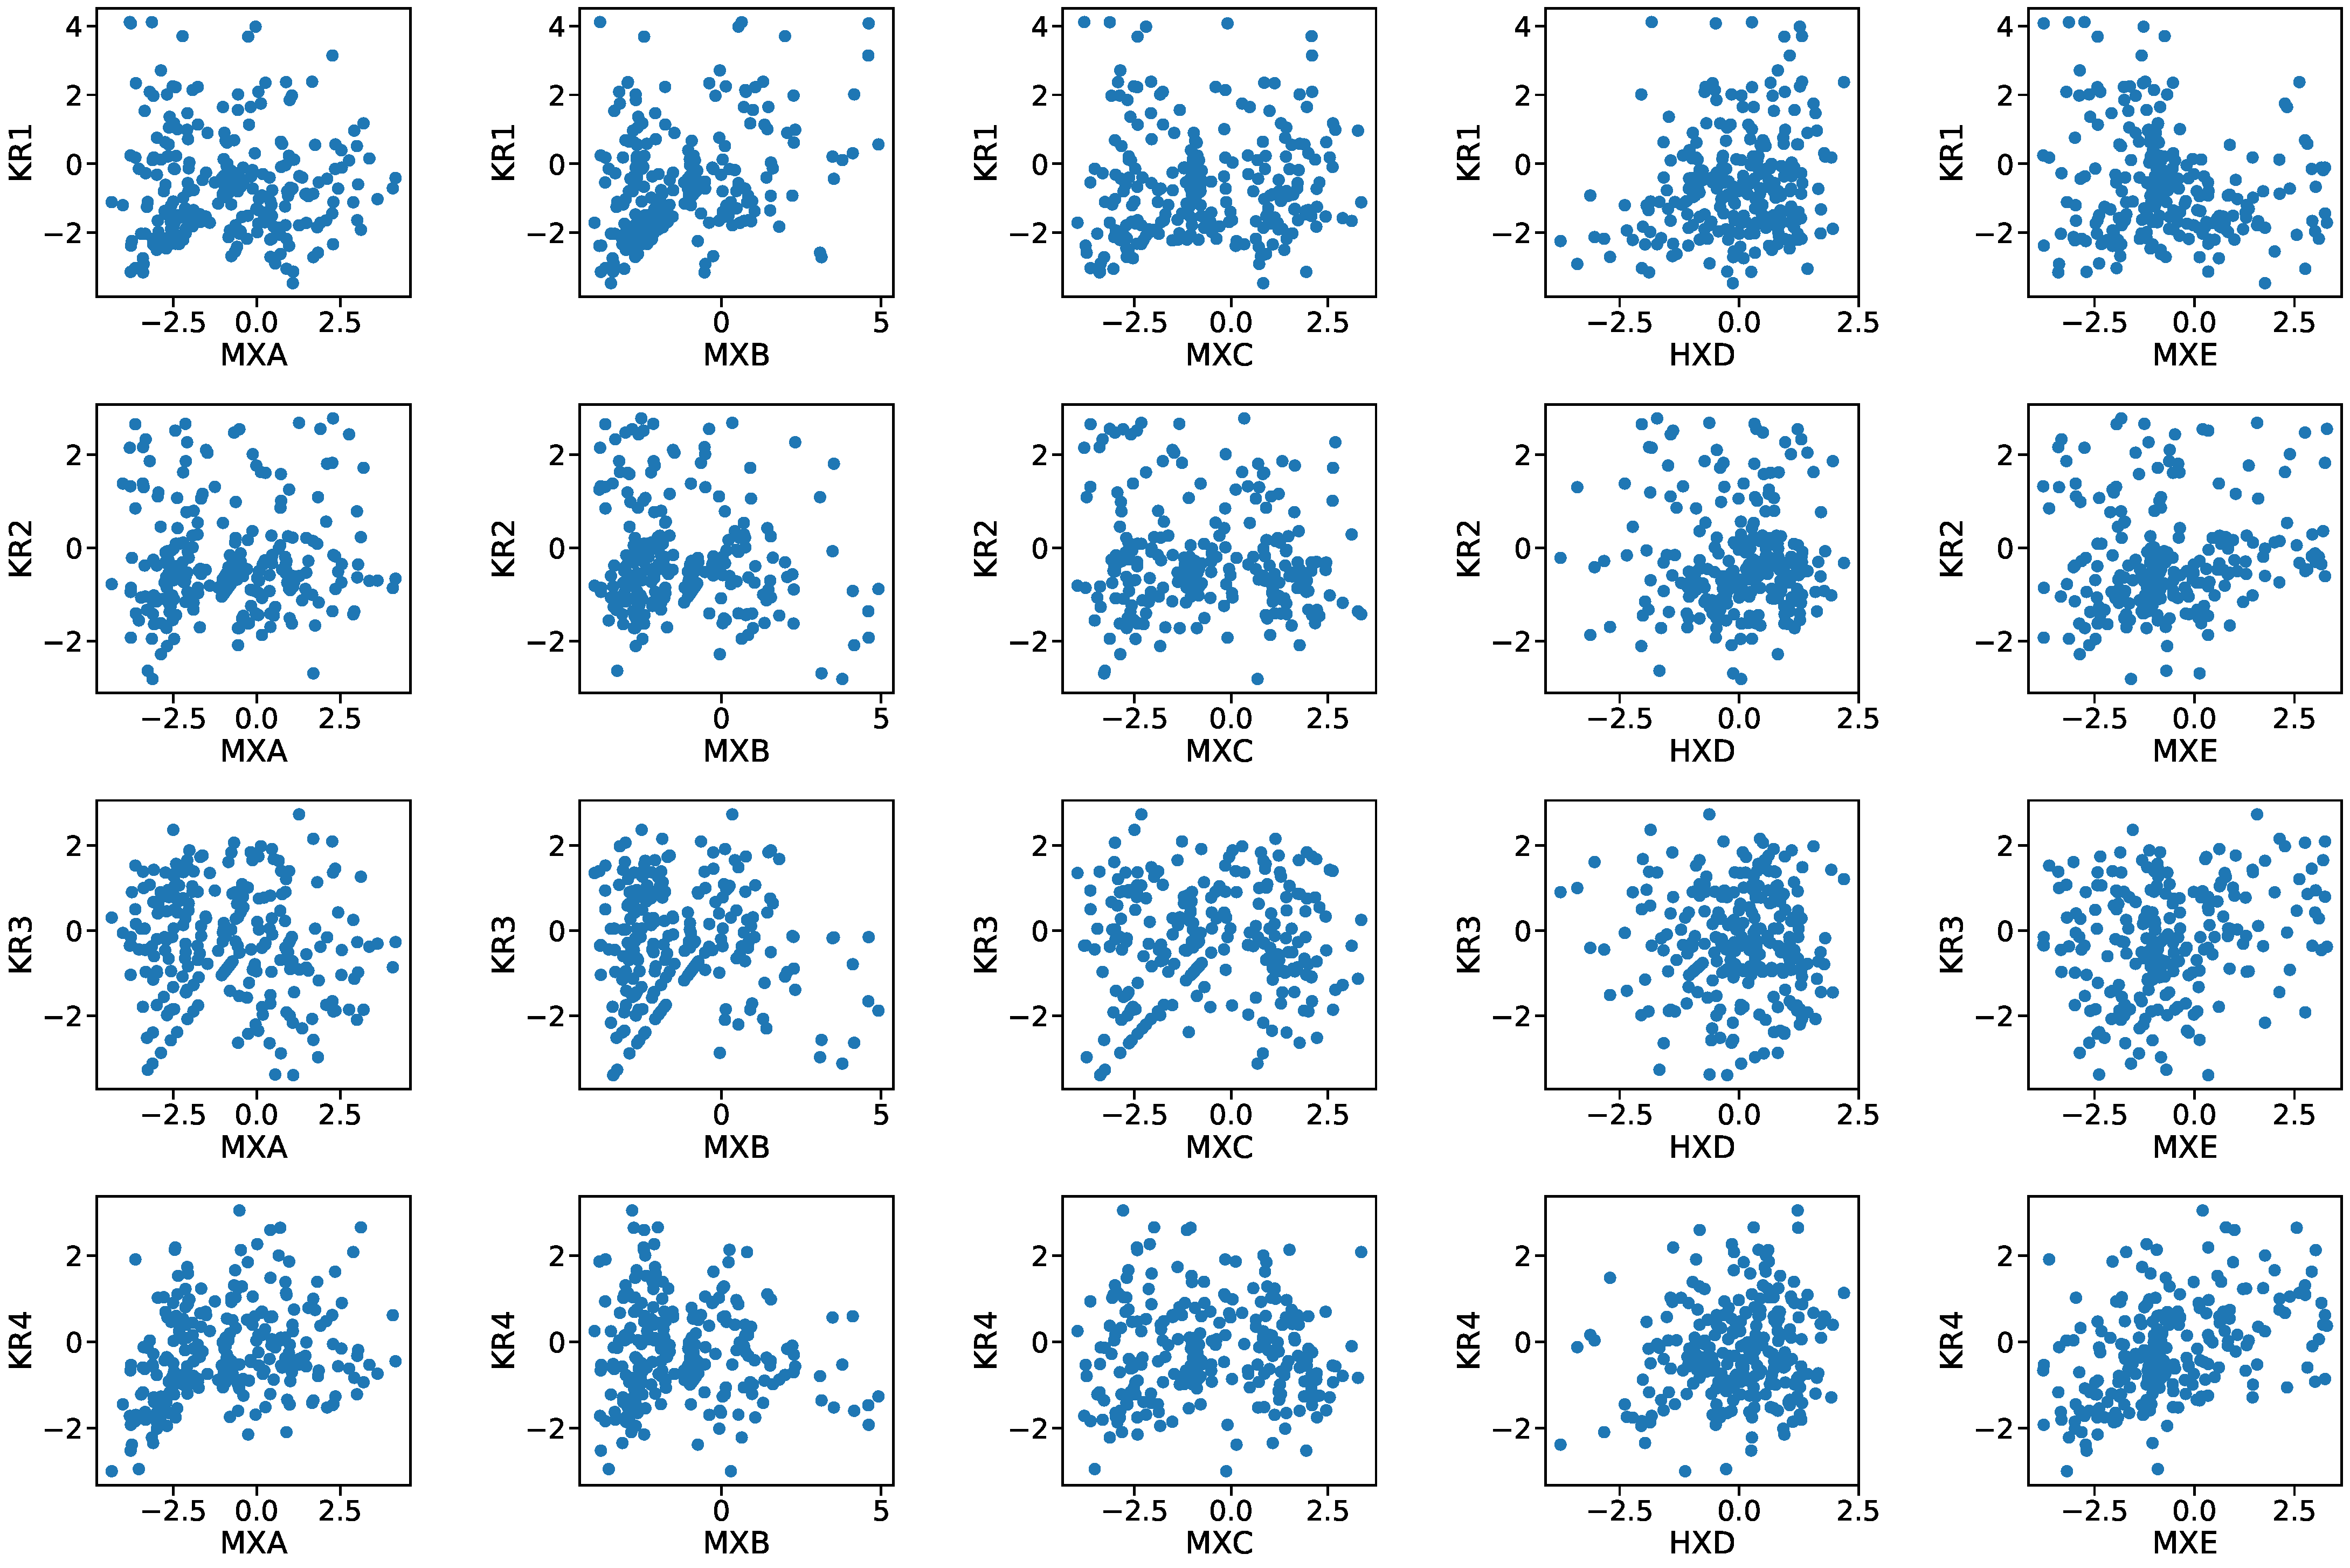
\includegraphics[width=\textwidth]{images/9_figs.pdf}
\caption{ length normalizing, multiply 1000 (rows sum to 1000), add 1, log}
\label{fig:9plots}
\end{figure}

\begin{figure}[h]
\centering
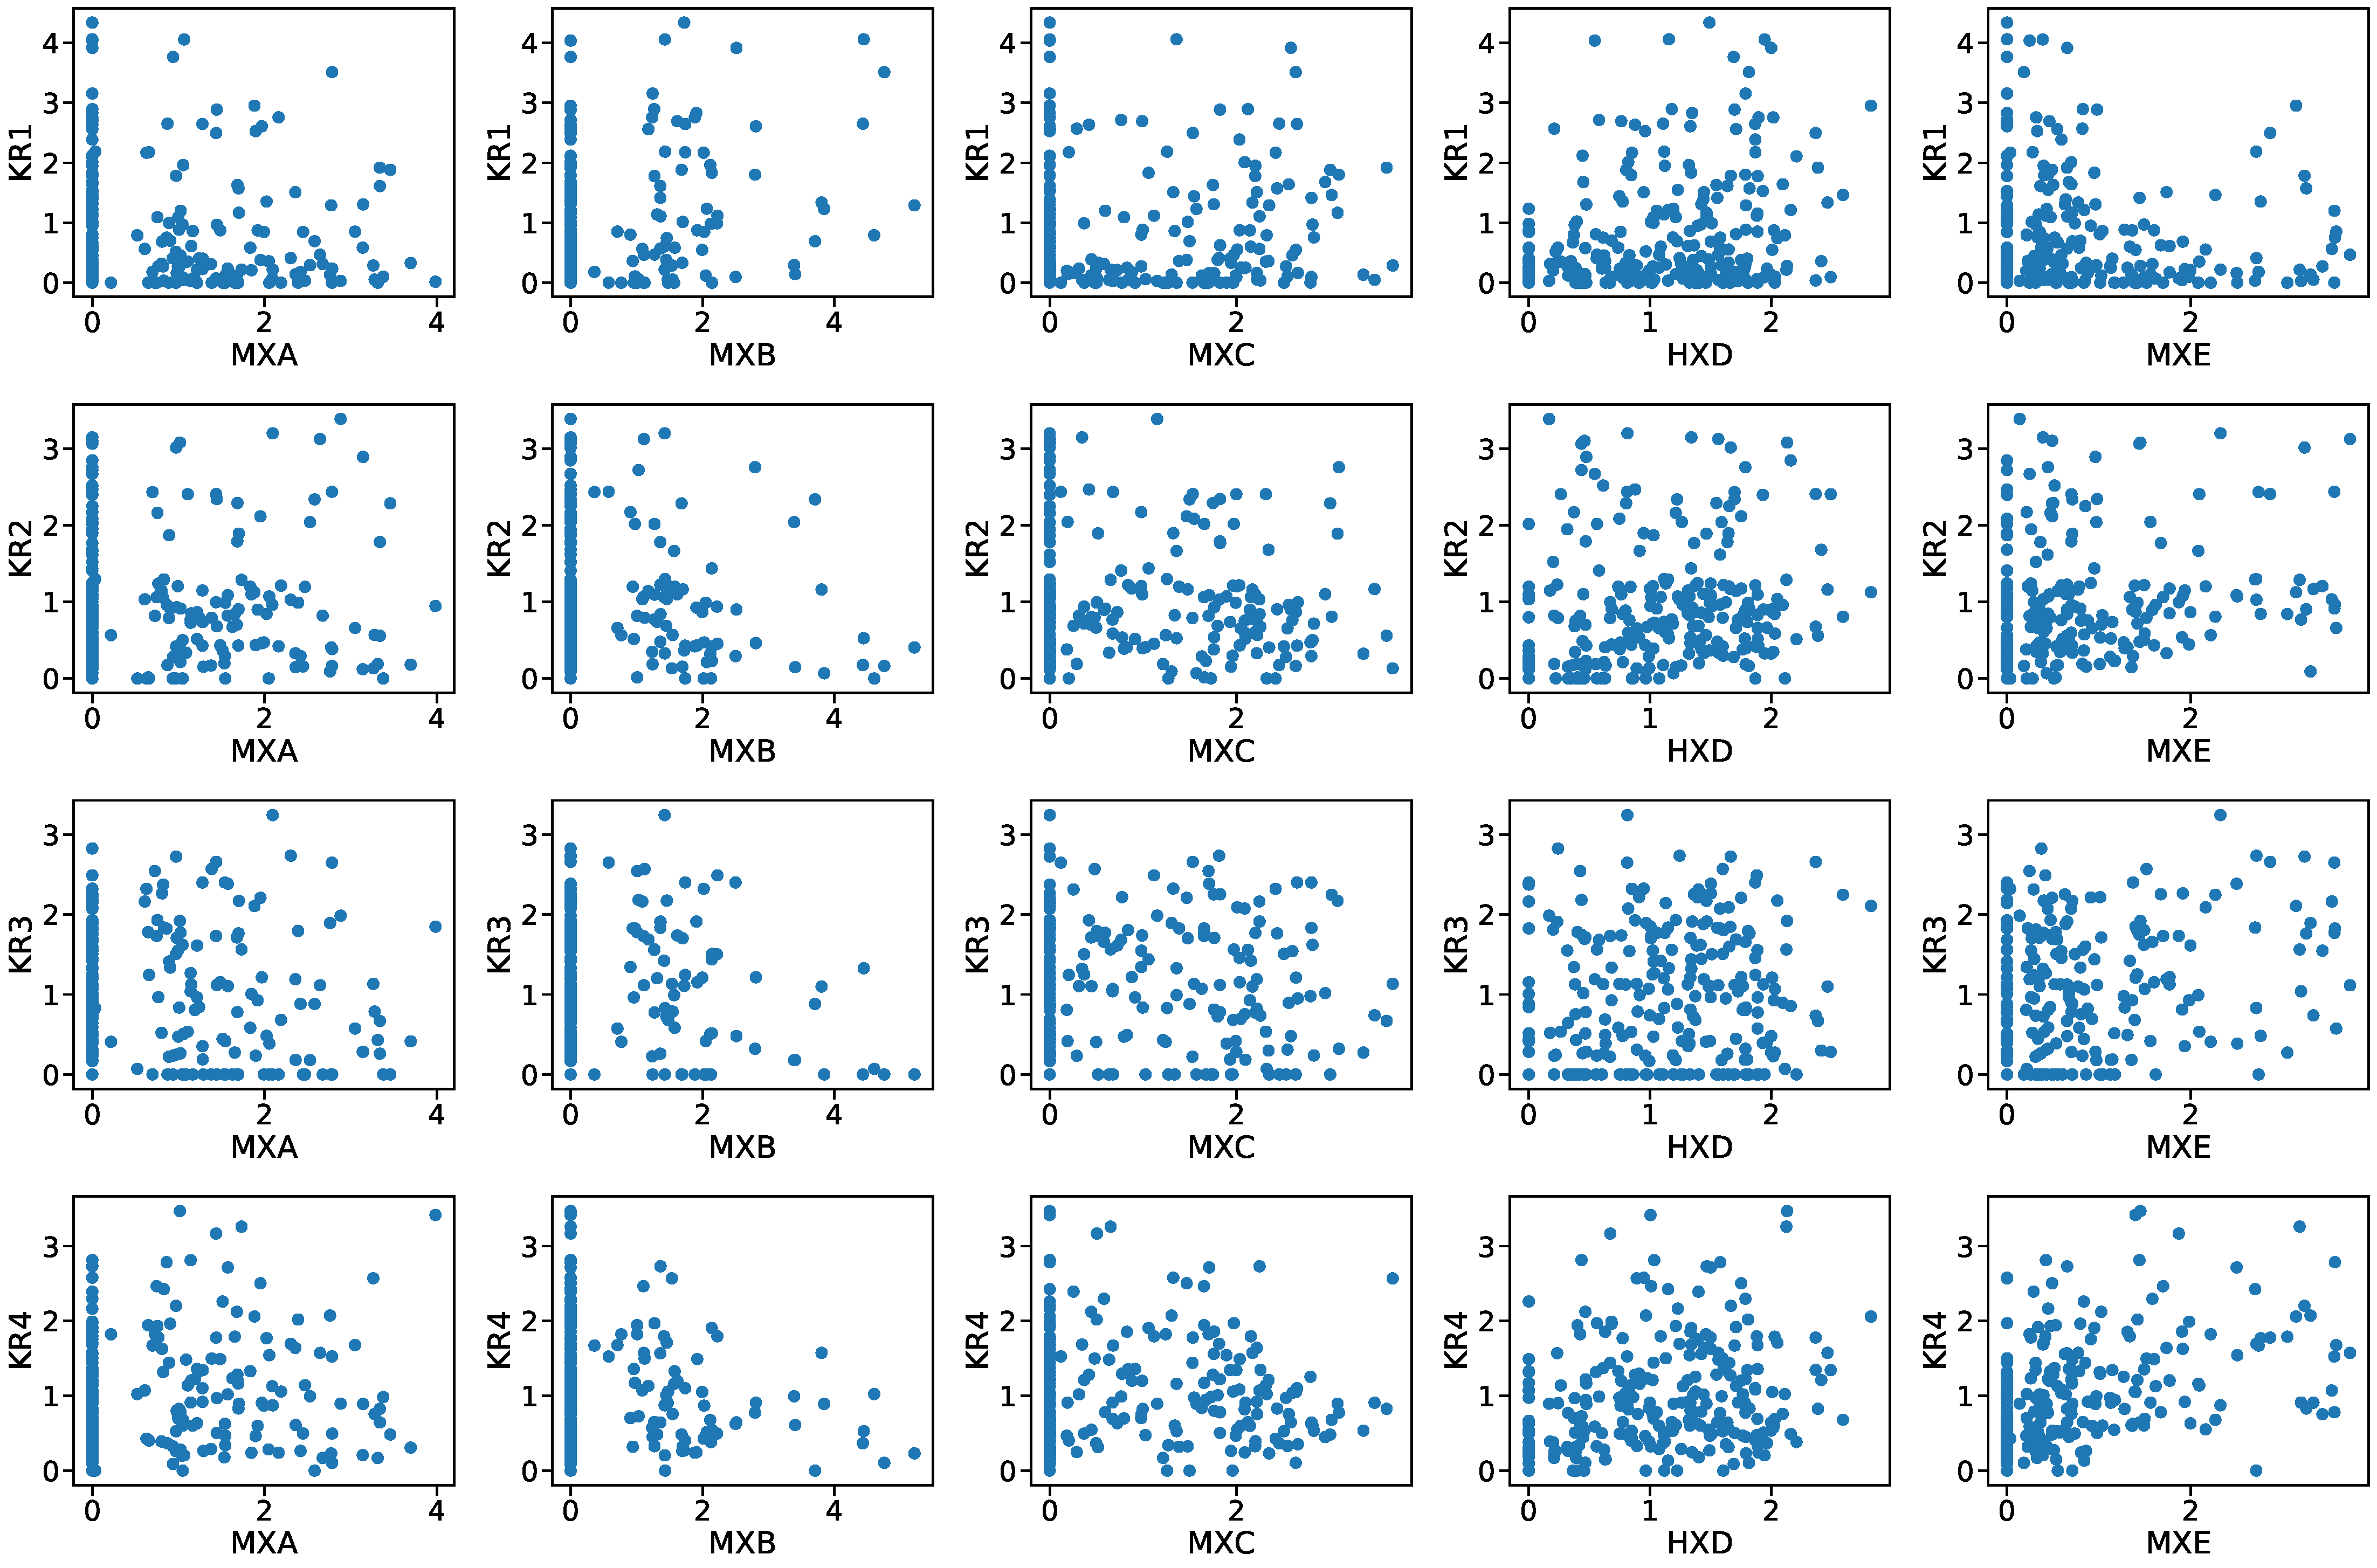
\includegraphics[width=\textwidth]{images/2_figs.pdf}
\caption{z-score column addition}
\label{fig:2plots}
\end{figure}
%\section{Methods}
